\documentclass{memoir}
\usepackage[english]{babel}
\usepackage[T1]{fontenc}
\usepackage[utf8]{inputenc}
\usepackage{natbib}%[doi=false,isbn=false,url=false,eprint=false,natbib=true]
\bibliographystyle{unsrtnat}
\usepackage{listings}
\usepackage{graphicx}
\usepackage{changepage}
\usepackage{amsmath}
\usepackage{lstautogobble}
\usepackage{hyperref}
\lstset{tabsize=2}

\usepackage[%
    left=1in,%
    right=1in,%
    top=1.0in,%
    bottom=1.0in,%
    paperheight=11in,%
    paperwidth=8.5in%
]{geometry}%


\title{Enhanced Sampling Techniques}
\begin{document}


\date{}

\maketitle

\tableofcontents

\chapter{Running All-Atom Molecular Dynamics Simulations of Intrinsically Disordered Proteins with Replica Exchange Solute Tempering Methods}
\chapterprecis{Jaya Krishna Koneru and Korey Reid, and Paul Robustelli}

\section{Abstract}
Accurate simulations of intrinsically disordered proteins and peptides  predictive power and insight into experimental findings extending our predictive capabilities in molecular interactions and understanding biological mechanisms. 
Unlike equilibrium simulations of ordered proteins in their ground state, simulating disordered proteins, as well as rare allosteric effects in structured proteins, require long continuous simulations which may not be well sampled even out to 1 ms. 
Replica exchange molecular dynamics simulations with solvent scaling proves to be a powerful group of methods to sample dynamics with limited resources. 
REST2 and ssREST3 are promising methods in accelerating the sampling of the conformational ensemble, not ommiting the caveat: the simulation is only as good as the forcefield. 
In addition to discussing the background, we provide an example of REST2 and ssREST3 as it pertains to simulating the C-terminal domain of $\alpha$-synuclein with and without a small molecular ligand and with an emphasis on assessing convergence of desired collective variables or observables. 

\textbf{Keywords} Molecular dynamics, Replica Exchange, Collective variables, Solute-Scaling, $\alpha$-synuclein

\section{Introduction}\label{sec:Intro}

% Your content goes here
    

Studying and critically understanding the underlying dynamics of biological systems at the atomistic scale can provide valuable insight into molecular mechanisms. 
Over many decades experimental techniques have been and continue to be developed in a collective effort to investigate processes at the molecular scale.
However, the limitations of experimental techniques often are restricted from producing clear and relevant explaintions at the atomistic level. 
This is in large part to the ensemble characteristic of experimental measurements and lends to the difficulty of extracting conformational dynamics at various timescales, as well as extracting localized dynamics of say a biological system. 
Upon entry of molecular dynamics the usefullness was apparent, albiet limited by computational speed. 
As molecular dynamics engines\cite{Weiner1981,gotz2012,salomon-ferrer2013,Brooks1983,Brooks2009,VanDerSpoel2005} and their accompanied forcefields\cite{Huang2016,Ploetz2021,Cornell1995,lindorff-larsen2010,Robustelli2018,Jakobsen2015,Piana2020} have matured, our ability to reach microsecond timescales has become routine. 
While the product of many decades of effort have resulted in our ability to simulate microseconds for a single biomolecule, vastly extending our comprehension of atomistic dynamics when paired with experimental results, these timescales are in fact beneath the threshold required to study rare events, e.g. allosteric transitions, or sample large degrees of freedom often accompanying IDPs. 

When the desire is to study conformational dynamics it becomes a neccessity for long-timescale simulations on supercomputing systems\cite{Shaw2009,Shaw2014}, for all other cases where statistical measures of an ensemble enhanced sampling techniques are available\cite{Lee2016,Wang2011,Qi2018,Vitalis2009,Zhang2023,Ray2023,Prakash2018}. 
%We need to append a reference to using enhanced sampling to produce starting conformations for unbiased simulation series plues references to others have done so. 
The phenomenological observation desired dictates which simulation methodology will provide usefull information.
One such method, Replica Exchange Solute Tempering or REST\cite{Liu2005,Wang2011,Zhang2023}, has arrisen from Hamiltonian Replica Exchange Molecular Dynamics (HREMD) a derivative of Replica Exchange Molecular Dynamics (REMD). 
For each of these methods, multiple parallel simulations are conducted in parallel. 
These parallel simulations undergo exchanges at a designated interval.
The relevance differences in each exchange method is discussed in the Introduction and Theory section, for a detailed account please refer to the original publications\cite{Sugita1999,Liu2005,Wang2011}.
 
\subsection{Replica Exchange Theory}
From Replica Exchange Molecular Dynamics\cite{Sugita1999}, the hamiltonian representing the potential energy of the system can be written as sum of respective contributions, separated into protein-protein, protein-water and water-water:
\begin{center}
    \begin{equation}
        E_{n}^{REMD}(X_{n}) = \lambda_{n}^{pp} E_{pp}(X_{n}) + \lambda_{n}^{pw} E_{pw}(X_{n}) + \lambda_{n}^{ww} E_{ww} (X_{n})
    \label{eq:remd_hamiltonian}
    \end{equation}
\end{center}

$\lambda_{n}^M$ is the scaling factor, where $M=\{ pp, pw, ww\}
$ which scales the corresponding energy term. For REST2\cite{Wang2011}, $\lambda_n^{ww}=1$, $\lambda_n^{pp}=(\lambda_n^{pw})^2=\lambda_n$, for simplicity the REST2 hamiltonian simplifies to:
% import simplified hamiltonian of REST2
\begin{center}
    \begin{equation}
        E_{n}^{REST2}(X_{n}) = \lambda_{n} E_{pp}(X_{n}) + \sqrt{\lambda_{n}} E_{pw}(X_{n}) +  E_{ww} (X_{n})
        \label{eq:rest2_hamiltonian}
    \end{equation}
\end{center}
% import lambda scaling equation
where,
\begin{center}
    \begin{equation}
        % \lambda_{n}^{pp}=\frac{\beta_{n}}{\beta_{0}} \ ; \quad \lambda_{n}^{pw}=\sqrt{\frac{\beta_{n}}{\beta_{0}}} \ ; \quad \lambda_{n}^{ww}=1;   
        \lambda_n = \frac{\beta_{n}}{\beta_{0}}
    \label{eq:lambda_scaling}     
    \end{equation}
\end{center}
% import temperature factor expression
and $\beta_{n}=\frac{1}{k_{B}T_{n}}\ for\ n=\{0,1,2,\ldots,n_{replica}\}$. 

Upon implementation of metropolis acceptance criteria with detail balance being satisfied, the acceptance probability between state $n$ and $n+1$ is given by:
\begin{center}
    \begin{equation}
        \Delta_{n,n+1} = (\beta_{n} - \beta_{n+1}) \Big[(E_{pp}(X_{n+1}) - E_{pp}(X_{n})) + \frac{\sqrt{\beta_{0}}} {\sqrt{\beta_{n}}+\sqrt{\beta_{n+1}}} (E_{pw}(X_{n+1}) - E_{pw}(X_{n}))\Big].
        \label{eq:rest2_AR}
    \end{equation}
\end{center}

By excluding the solvent-solvent interactions w.r.t. scaling, the contribution to the acceptance criteria contains less degrees of freedom relative to REMD resulting in better acceptance between replicas.

Upon investigation, disordered proteins containing hydrophobic residues undergo conformational collapse with respect to scaling  $E^{pw}$ to higher effective temperatures. 
This outcome is unfavorable when attempting to capture a representative ensemble as hydrophobic collapse reduces the overall sampling of the proteins conformational ensemble. % We need to say something here to the effect: REST2's ability to enhance hydrophobic interactions is synonamous with reducing the quality of the solvent, water. 
\citeauthor{Zhang2023} \citeyear{Zhang2023} provided a basis for biasing the scaling such that protein collapse is minimized or negated, with the hamiltonian:
\begin{center}
    \begin{equation}
        E_{n}^{REST3}(X_{n}) = \lambda_{n} E_{pp}(X_{n}) + \kappa_n\sqrt{\lambda_{n}} E_{pw}(X_{n}) +  E_{ww} (X_{n}).
        \label{eq:rest2_hamiltonian}
    \end{equation}
\end{center}

%add in info about variables, what are they?
By incorporating the scaling factor $\kappa_n$, where $n=\{1,2,3,\ldots,n_{replica}\}$, the dampening effect of $\lambda$ is deminished. 
To accomplish this $\kappa_n$ exist in the range $[1.0,1.06]$. 
Due to the method of implementation the base replica (unscaled topology), following conversion of the topologies to REST3 \cite{Zhang2023} formalism using combination rule 1 instead of 2, does not match the potential energy of the original topology. 
The implementation of REST3 by \citeauthor{Zhang2023} target scaling of protein-water lj parameters by means of computing C6 and C12 parameters. 
There exists a descrepancy between the unscaled-converted topology and the original topology via machine error of switching the potential from combination rule 2 to combination rule 1 in GROMACS, however, the conformational sampling desired is observed. When $\lambda$ scaling is applied, as in REST2, the well depth of the LJ potential is deminished, Figure 
\begin{figure}
    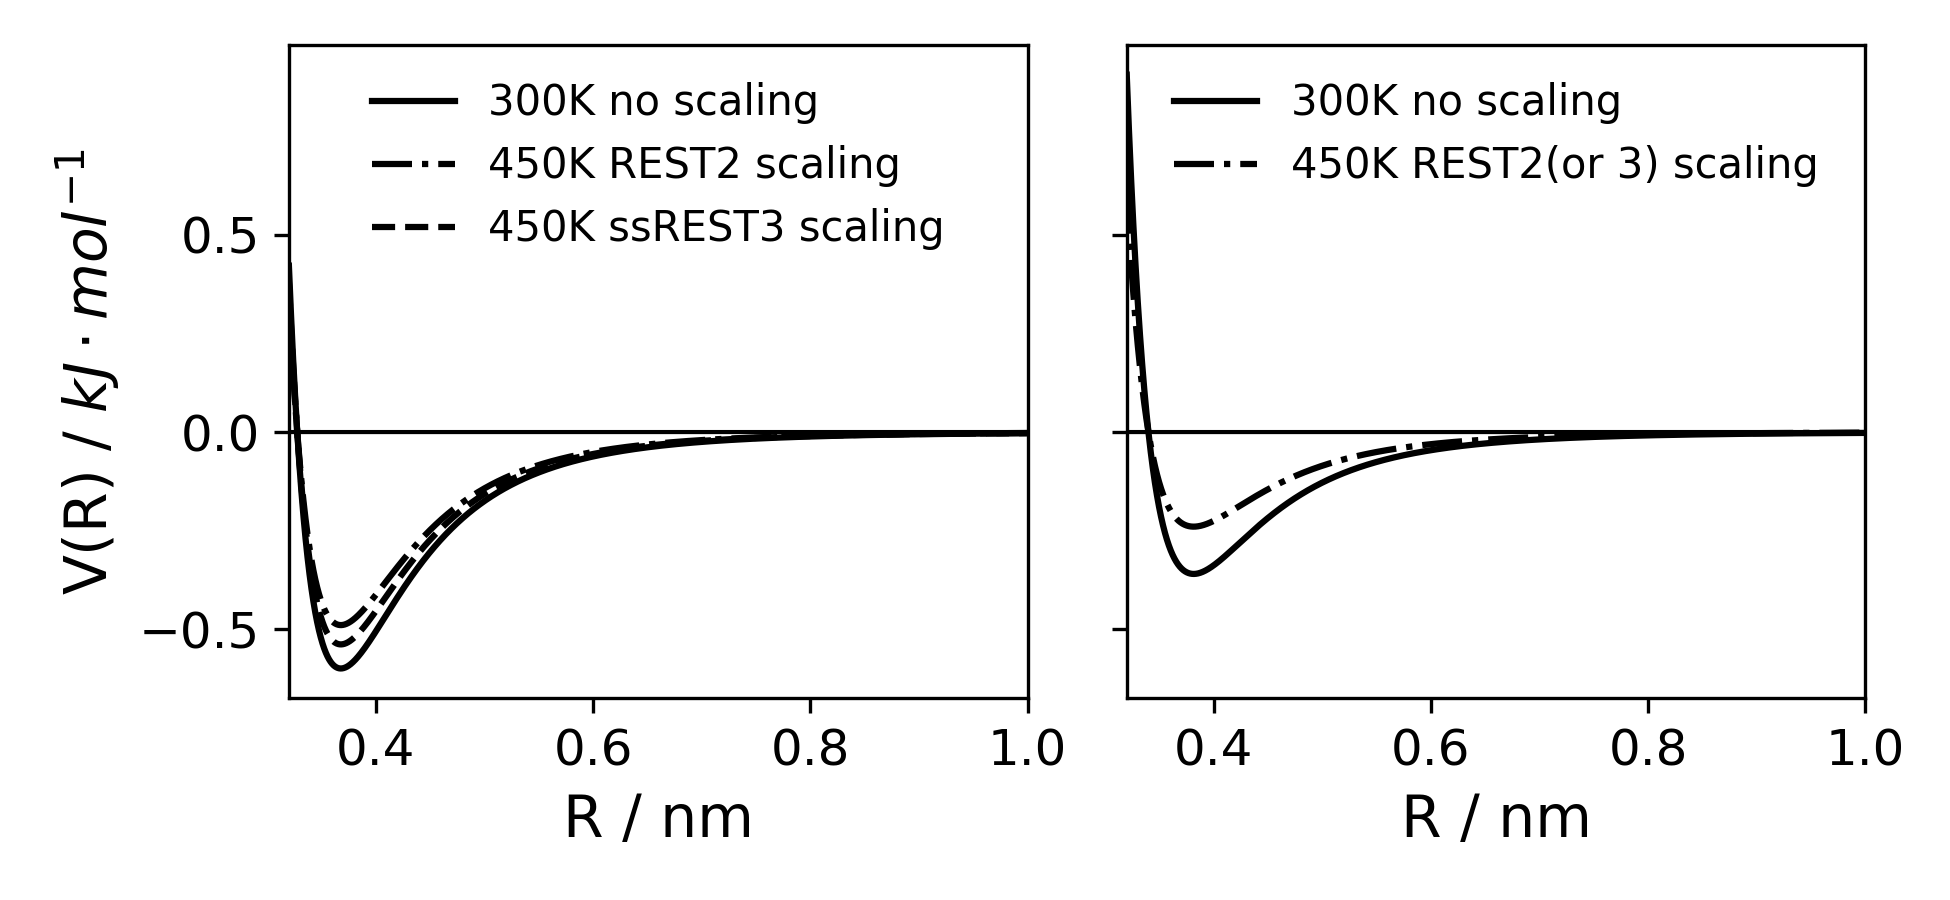
\includegraphics[width=\textwidth]{../Figure_a/fig_a.png}
    \caption{LJ potential for differing values of epsilon for the same atom-atom pair.}
    \label{fig:lj_curves}
\end{figure}
where $\lambda_n$ is still applied to the protein in the same fashion as REST2 \cite{Wang2011} and solvent scaling is applied to the water oxygen via the well-depth, $\epsilon_{OW}$, borrowing from the methods described in \citeauthor{Best2010} \citeyear{Best2010}. 
To overcome the inherent mechanics within GROMACS\cite{VanDerSpoel2005}, nonbonded overrides are implemented for water-water and water-ion.
Additionally, one can override water-cosolute if scaling is not desired between the two. 
For ssREST3, $\kappa_n$ is defined by the expression, 
\begin{center}
    \begin{equation}
        \kappa_{n}=\kappa_{low}*\exp{ \biggl(n*\frac{\log(\kappa_{high}/\kappa_{low})}{N_{r}-1}\biggr)} \ ; \quad 1.00 \leq \kappa_{n} \leq 1.10.
    \label{eq:kappa_scaling}
    \end{equation}
\end{center}

To understand where $\kappa_n$ is applied, we start with an expression for the Lennard-Jones potential between the $i^{th}$ protein atom and the water oxygen,
\begin{center}
    \begin{equation}
        \sqrt{\lambda_n}\cdot\kappa_n\cdot E_{i,OW}^{lj} = \sqrt{\lambda_n}\cdot \kappa_n \cdot 4 \cdot\epsilon_{i,OW}\Big[ \Big( \frac{\sigma_{i,OW}}{r}\big)^6 -  \Big( \frac{\sigma_{i,OW}}{r}\big)^{12} \Big]
    \label{eq:lj_potential}
    \end{equation}
\end{center}

The CHARMM and Amber forcefields both conform to the Lorentz-Berthelot rules, i.e. $\epsilon_{i,j}=\sqrt{\epsilon_i\cdot \epsilon_j}$. From Equation \ref{eq:lj_potential} we can refactor $\sqrt{\lambda_n}\cdot\kappa_n\cdot\epsilon_{i,OW}$ to clarify which forcefield parameters are scaled. 
\begin{center}
    \begin{equation}
        \epsilon_{p:OW}=(\epsilon_{p:p}^{rescaled} * \epsilon_{OW:OW}^{rescaled})^{\frac{1}{2}}=\lambda_{n}^{pw}\kappa_{n}*(\epsilon_{p:p} * \epsilon_{OW:OW})^{\frac{1}{2}}
    \label{eq:wat_scaling}
    \end{equation}
\end{center}

The sections that follow are the Materials, Methods and Notes sections.
Within the materials sections we detail the required software and minimum hardware requirements to perform REST based simulations.
The Methods sections contains a complete description with examples on how to create and produce REST2 and ssREST3 simulations following an example simulation involving $\alpha$-synuclein and a small molecule. Additionally, we include a few examples of analysis to test for convergence. Lastly, we provide various Notes in the last section. 

\section{Materials}

For any simulations initial positions of the particles are very important.
PDB files provides us with the required information about the initial coordinates where each atom is represented as a particle in space.
It might get one wondering on how can a bunch of particles arranged in a 3-dimentional space can behave as a protein or a small molecule.
This is achieved with the help of force-field parameters which are a set of basic parameters that governs the interaction potentials between the different atoms of the molecule or protein.
These force-field parameters are derived and optimized from quantum mechanical calculations and experimental data which helps us in replicating the macroscopic observables.
There are many force-fields available fo both explicit and implicit solvent models.
For explicit solvent models, most commonly known force-fields are Amber99SB-ILDN$^{*}$,Amber99SB-\textit{disp}, CHARMM36m, OPLS-AA, GROMOS96, etc in which we will be using Amber99SB-ILDN$^{*}$ force-field as it has shown to reproduce the experimental ensembles of IDPs.
$\alpha$-synuclein is an intrinsically disordered protein which is known to be involved in Parkinson's disease and its C-terminal region made up of 20 amino acids will be our system of interest.
     

\section{Methods}
Now that we have a base understanding of Replica Exchange Methods it is high time to apply this new found knowledge. 
This example focuses on the application of REST2 on $\alpha$-synuclein in a solvated water box.
In the first part we will generate starting structures. In the second part, follwing generating the independent systems from our assortment of starting structures, each will be equilibrated, one for each replica. 
In the third part, from each equilibrated system the final configuration will carry forward and the paired topology will be scaled by $\lambda_n$ as described in Section \ref{sec:Intro-RE}, Eq. \ref{eq:lambda_scaling}. In the fourth part, simulations will be caried out with simple instructions to check if the systems are exchanging appropriately and a show of exchange convergence w.r.t. round trip times. In the last part, we will carry out an analysis on the resulting trajectory, which will include de-multiplexing of the temperature replica and convergence analysis. 
\subsection{Starting Structure Production}
There are many different methods for producing starting structures. We will opt to produce starting structures from an exteded chain for all $N_r$. 
\subsection{Equilbrating Independent Systems}
To equilibrate each system we will follow the general approach for equilibrating each system. 
It is important to note that REST2 simultions with plumed are performed under the canonical ensemble, NVT, thus it is of utmost importance that we equilibrate our box sizes so that our pressure at the base replica is near or on top of our desired system pressure. 
\subsection{Creating the REST2 Simulation Input}

Implementing REST(2 or 3) using the GROMACS\cite{VanDerSpoel2005} molecular dynamics engine requires installation of PLUMED2 plugin version$\ge2.8$ and patching of GROMACS source code before compiling mdrun. Please note that PLUMED2 can be used alongside the AMBER MD engine version$ge18$ and NAMD version$\ge2.12$ at a significant cost to performance. For a simple walkthrough of this installation procedure for GROMACS please refer to Note \ref{notes:installation}.
%We need to discuss REST2 generation first, then state added edits to produce ssREST3
The first step in the ssREST3 implementation is to generate the a processed topology file your solvated protein of interest using \textit{-pp} option in \textit{gmx grompp}, note any position restraints contanted in an mdp file will be contained in the processed topology file.

\begin{lstlisting}[language=sh, basicstyle=\ttfamily\small, breaklines=true]
    gmx grompp -f *.mdp -c *.gro -r *.gro -p topol.top -o *.tpr -pp
\end{lstlisting}

\noindent This topology files will be used as to implement REST2 scaling procedure using PLUMED2.8 where one will supply the processed topology file and the corresponding $\lambda$ value as such :

\begin{lstlisting}[language=sh, basicstyle=\ttfamily\small, breaklines=true,escapeinside={(*}{*)}]
    plumed partial_tempering   (*$\lambda_{n}$*) < processed.top > scaled.top
\end{lstlisting}

After the topology files are generated for the respective replicates, the oxygen atom 
of the solvent, for example OW$_{tip4pd}$ which is the water oxygen atom of amber99sb-\textit{disp} force field, will have $\epsilon$ scaled by a factor of $\kappa^{2}_{n}$ to satisfy the scaling condition, 
 Eqs. \ref{eq:kappa_scaling} and \ref{eq:wat_scaling}. 
If $\kappa_{n}$ is set to 1.0 across all replicas the topologies conform to the REST2 convention. 
Along with the scaling of the water oxygen, we recover the interactions between the solvent molecules, and between solvent and ions, thus targeting only the protein-water LJ potential. 
This is accomplished by adding three non-bonded overrides to the \textit{[nonbonded]} section of the GROMACS topology file as shown in Table \ref{tab:eps_noscale_table}.
Once these changes are made to the topology, we are ready to simulate ssREST3.
Using the below command all the replicates are run in parallel and the the conformational exchange between the replicas is set for every 800 steps which equates to 1.6 ps.

\begin{lstlisting}[language=sh, basicstyle=\ttfamily\small, breaklines=true]
    gmx  grompp -f *.mdp -c *.gro -r *.gro -p scaled.top -o scaled.tpr
    gmx mdrun -s scaled.tpr -multi <replica folders> -replex 800 -deffnm replica -plumed plumed.dat
\end{lstlisting}


At the start of the simulations it is best practice to check the acceptance ratios between replicas to ensure that the scaling is not too aggressive nor too weak. 
A minimum of 20\% acceptance ratio is recommended for the simulations to be considered valid.
\subsection{Running a REST2 Simulation}
We use C-terminal of $\alpha$-synuclein in presence of a ligand called "Fasudil" and use REST2 and REST3 enhanced sampling techniques to simulate with our base temperature at 300K 
and 450K as maximum temperature to generate the temperature ladder.
We made sure that the terminal capping is done for the 20 amino acid peptide.
We generate 10 replicates for REST2 and 8 replicates for REST3 simulations.
The protein is solvated in a 6.5 nm cubic box using tip4p-\textit{disp} a 4 point water model which has shown good agreement with IDP's and sufficient amount of NA$^{+}$ or CL$^{-}$ ions are added to netralize the 
system.
The system is energy minimized up to 5000 steps using steepest decent algorithm and then system has undergone a rigorous equilibration.
After a successful minimization the system is heated up to 300K under NVT ensemble for 500ps coupled to a temperature bath using V-rescale algorithm.
Once the solvated system is heated up, the system undergoes a 100ps equilibration under NPT ensemble where it is coupled with Berendsen barostat so that the pressure of the system 
is maintained at 1 bar.
Berendsen barostat helps in a quick convergence of pressure towards 1 bar after which we equilibrate under NPT condition for another 40ns using Parrinello-Rahman barostat which 
helped the system to achieve a convergence around 1 bar of pressure.
After the pressure was well converged the last frames of the replicas are used as a staring configurations for REST2 and REST3. 
The replicates are simulated under NVT ensemble for 1.98$\mu$s and 1.3$\mu$s totaling an aggregate of 19.8$\mu$s and 10.4$\mu$s for REST2 and REST3 ensembles.
Radius of Gyration which gives us an estimate whether the protein is collapsed or elongated is used as a metric and its distribution is computed using MDTraj after the trajectories 
are corrected for there periodicity.
As shown in the Fig : we can see that the protein ensemble simulated using REST3 stays elongated when compared to REST2 as there is a positive shift in the distribution of 
$\alpha$-carbon Rg. 


\subsection{Performing Analysis}
Analysis is important, JK take it away!

\section{Notes}

\begin{enumerate}
\item Basic installation of plumed and gromacs with openmpi preinstalled on a Linux system with the gcc compiler in a bash environment. 
This series of commands assumes you have the variable \$MPICXX set. 
Further gains in performance can be reached by utilizing multiple NVIDIA GPUs and the CUDA compiler, nvcc, and the cude runtime. Detailed descriptions on compiling GROMACS and PLUMED2 can be found at \href{http://gromacs.org}{http://gromacs.org} and \href{http:/plumed.org}{http:/plumed.org}, respectively.\\
    \begin{minipage}[t]{\linewidth}
        \begin{lstlisting}[language=bash,xleftmargin=0mm,autogobble,breaklines=true]
            #!/bin/bash
            INSTALL_ROOT=$HOME/opt
            mkdir src
            cd src
            git clone https://github.com/plumed/plumed2.git
            git clone https://github.com/gromacs/gromacs.git
            cd gromacs
            GMX_version=2024.3
            git checkout -b v$GMX_version$
            cd ../plumed2
            ./configure --prefix=$HOME/opt --enable-modules=all CXX="$MPICXX" CXXFLAGS="-O3 -axSSE2,AVX" 
            make
            make check
            make install
            echo 'export PLUMED_KERNEL="/usr/share/lib/libplumedKernel.so"' >> ~/.bashrc
            echo 'export PATH=$HOME/opt/bin:$PATH' >> ~/.bashrc
            echo 'export PLUMED_ROOT=$HOME/opt'
            source ~/.bashrc
            cd ../gromacs
            plumed patch -e gromacs-${GMX_version}
            mkdir build
            cd build
            cmake .. -DGMX_THREAD_MPI=OFF -DGMX_MPI=ON -DGMX_BUILD_OWN_FFTW=ON -DREGRESSIONTEST_DOWNLOAD=ON -DCMAKE_INSTALL_PREFIX=$HOME/opt
            make 
            make check 
            make install
        \end{lstlisting}
    \end{minipage}\label{notes:installation}
\end{enumerate}

\begin{table}[h!]
    \centering
    \caption{Table showing the differences and similarities of $\epsilon$ scaling between the REST2 and ssREST3 methods. In case of ssREST3 the 
    water $\epsilon$ gets scaled along with the solute $\epsilon$ by a factor if $\kappa^{2}$ where as solvent parameters are not scaled during REST2.}
    \begin{tabular}{c | c c c c c }

    Method & $T_{max}(K)$ & $\lambda$ & $\epsilon_{CA}$ & $\kappa$ & $\epsilon_{OW}$ \\
    \hline
    -- & 300 & 1.0 & 0.359824 & 1.0 & 0.998989 \\
    REST2 & 450 & 0.666667 & 0.239883 & 1.0 & 0.998989 \\

    ssREST3 & 450 & 0.666667 & 0.239883 & 1.1 & 1.20878 \\
    
    \hline
    \end{tabular}
    
    \label{tab:eps_table}
\end{table}
\begin{table}[h!]
    \centering
    \caption{Table with $(\sigma_{ij}, \epsilon_{ij})$ showing the solvent interactions with itself and ions remain unaffected by the scaling factor $\kappa_{n}$.}
    \begin{tabular}{c | c c c }

    Atom types & OW$_{tip4p}$ & NA$^{+}_{C22^{*}}$ & CL$^{-}_{C22^{*}}$ \\
    \hline
    OW$_{tip4p}$ & (0.3165, 9.98989) & (0.279746, 0.442754)  & (0.360484, 0.791812)\\
    
    \hline
    \end{tabular}
    
    \label{tab:eps_noscale_table}
\end{table}

\section{Acknowledgements}
I thannk blah blah for the blah blah to the blah blah, edit this for sure.

\bibstyle{unsrtnat}
\bibliography{enhanced_sampling.bib}
\end{document}
